\glsresetall
\chapter{Introduction}	\label{ch:introduction}
The simulation of combustion processes poses a significant computational challenge, mainly due to the intricate interaction between chemical reactions and fluid dynamics. The complexity arises from the inherent nature of combustion processes, which often involve multiple simultaneous chemical reactions. These reactions release energy in the form of heat, leading to the formation and propagation of flames. At the same time, fluid dynamics largely drives the transport of heat, mass and momentum, which in turn influences the behavior of the flames.  To accurately capture these phenomena, computational models must consider thermodynamic aspects, and properly represent the chemical reactions, species transport and fluid flow involved. These processes are highly nonlinear, rendering their numerical representation difficult.

Of particular interest for many practical applications is the simulation of diffusion flames, which is the result of the combustion of initially separated oxidizer and fuel. The use of numerical methods to simulate diffusion flames can offer crucial insights into flame structures and combustion efficiency. Recently \Gls{DG} methods have demonstrated high accuracy and efficiency for simulating combustion processes. In this thesis, a fully coupled \gls{DG} method for simulating diffusion flames will be developed. To explore the method's suitability various simulations will be analysed.

\section{The \Gls{DG} method for reacting flows}
The field of \Gls{CFD} has become a crucial tool for understanding and predicting complex fluid flows. Through the use of numerical methods and specialized algorithms, CFD allows researchers to simulate fluid dynamics problems and gain detailed insights into the behavior of fluids in motion. Detailed information about flow physics that is often difficult or impossible to obtain through experiments can be provided by these methods, leading to deeper insights into the mechanisms governing fluid flow. 

In addition to their scientific value, numerical methods for solving the governing equations of fluid dynamics have numerous practical applications. For example, the use of computational tools has become an essential step in the development of new products. They are widely used in fields such as the automotive, chemical and aerospace sectors, to name a few. They are also crucial for assessing the safety and reliability of systems such as chemical and nuclear reactors.

Historically speaking, the methods used in the early days of CFD were low-order numerical methods, such as \gls{FVM} or \gls{FEM}. These kind of methods use lower order polynomial functions to approximate the solution of the governing \glspl{PDE}. Although they are widely used and very well established, they can suffer from  low accuracy or difficultly in representing complex geometries. On the other hand, the so called high order methods use higher order polynomial functions to approximate the solution, allowing them to capture sharp gradients and complex flow structures with greater fidelity. While high-order methods are often more computationally expensive than low-order methods, they offer advantages when high accuracy is required. It should be noted that the \Gls{FVM} and \Gls{FEM} have also been extended to obtain higher order convergence.

High-order methods have been used since the early days of numerical simulation, but their use was limited due to their comparatively high computational cost. With the advent of modern high-performance computing systems and algorithms, the use of high-order methods has become more widespread and accessible. Today, high-order methods are widely used in many areas of computational fluid dynamics, including aerospace \parencite{mavriplisProgessHighOrderDiscontinuous2009}, automotive \parencite{colomboAssessmentDiscontinuousGalerkin2021}, and biomedical engineering \parencite{fehnModernDiscontinuousGalerkin2019}, among others. One of the most prominent methods is the so-called \gls{DG} method, which is the subject of this thesis.

\subsubsection{The \Gls{DG} method}
The \gls{DG} method is a numerical method to solve differential equations. It was initially developed for solving hyperbolic conservation equations, and has recently gained increased attention in the \gls{CFD} community. The key feature of the method is the use of a piecewise polynomial approximation of the solution field on each element of a computational mesh. This allows for high accuracy and flexibility, with the order of the polynomial being an adjustable parameter. 
The DG method combines the locality of low-order schemes with the accuracy per \gls{DOF} of spectral schemes. This feature allows for achieving the same level of accuracy as a low-order scheme with fewer \glspl{DOF}, leading to more efficient and computationally feasible solutions.  Another advantage of the  DG method is that is well suited to parallel computing. Within the DG method any given cell of the grid only requires information from its immediate neighbors, allowing an efficient parallelization with minimal communication overhead.

Additionally, in the DG method, the solution is allowed to be discontinuous across element boundaries, enabling the handling of complex geometries and solution discontinuities in a natural way. The conservation of a physical quantity (such as mass, momentum, or energy)  is ensured by construction in the DG method. This is achieved through the use of numerical fluxes, which approximate the flux of the conserved quantity at each element boundary. The numerical fluxes must meet certain stability and accuracy criteria to ensure the overall stability and accuracy of the method. 

%Additionally, the DG method is capable of handling under-resolved flows \parencite{henninkLowMachNumberFlow2022}. 

%\subsubsection{How does the Discontinuous Galerkin method compare to other methods?}
Compared to more popular methods such the \gls{FEM} and \gls{FVM}, the DG method offers several advantages. First, The DG method provides an arbitrary order of error convergence through the local polynomial approximation of the solution field. Specifically, a polynomial approximation of degree $p$ can achieve a numerical discretization error of order $\mathcal{O}(h^{p+1})$ for smooth solutions, where $h$ is a characteristic grid length. This contrasts sharply with other well established schemes, which are usually restricted to an accuracy of $\mathcal{O}(h^N)$, with $N \leq 2$ for unstructured grids. Second, the discontinuous approximation of the solution in the DG method allows for a robust treatment of discontinuities in the solution, which can be challenging for the classical \gls{FEM}. However, the DG method has the disadvantage that usually memory requirements  and overall computational costs are higher than in a finite element method.

\subsubsection{Diffusion flame modeling and the \Gls{DG} method}
Diffusion flames, also known as non-premixed flames, present a significant challenge for simulation due to their complex nature. These flames involve the mixing of two or more reactants before combustion can occur, resulting in a complex interplay of fluid dynamics, heat transfer, and chemical reactions. Moreover, diffusion flames are characterized by steep gradients in temperature, density, and species concentration, necessitating a high spatial mesh resolution for accurate simulation. In a diffusion flame, the reactants are initially separated, and their mixing is essential for combustion to take place. High-order methods, such as the DG method, offer a solution to alleviate the computational burden associated with the demanding numerical resolution required for accurate simulations.
 
A proper computational representation of a diffusion flame requires a suitable description of the combustion processes. Representing the involved chemical reactions in a accurate and efficient way poses a significant challenge. Although a detailed description of the chemistry is preferred, it can be computationally intensive and impractical due to the high number of chemical species and chemical reactions taking place. To overcome this issue, simplified kinetic models have been developed, such as the one step kinetic model presented by \textcite{fernandez-tarrazoSimpleOnestepChemistry2006} for hydrocarbon combustion with air, and is the model used in the present work. This model correlates kinetic parameters with the equivalence ratio, allowing for better representation of the characteristic flame properties of premixed and non-premixed flames. By using a single chemical equation, this model enables the study of complex combustion phenomena while substantially reducing the computational cost. Furthermore, it offers a straightforward and flexible approach to simulate phenomena that would otherwise require a more complex chemical model, such as the calculation of flame temperatures, or the simulation of reactant leakage and near-extinction diffusion flames.
 
The flow regime is also an important point to be addressed. Many practical applications of diffusion flames involve deflagration flames, which are combustion systems defined by a small characteristic flow velocity compared to the speed of sound  \parencite{poinsotTheoreticalNumericalCombustion2011}. To accurately model this type of system, the low-Mach approximation of the Navier--Stokes equations is often used. This approximation allows for the calculation of non-constant density flows while also neglecting acoustic effects, which also reduces the required temporal resolution. Explicit time marching algorithms are commonly used for simulations of deflagration flames using the low-Mach approximation, which enables a larger time step size and reduces computational time. However, implicit schemes can also be useful for simulating diffusion flames \parencite{mullerLowMachNumberAsymptoticsNavierStokes1998}, enlarging even more the allowed time-steps for obtaining an accurate simulation. 
\subsubsection{Solution of the governing system of equations}
Various solution strategies are available for solving the governing differential equations of fluid flow problems, which can be categorized into segregated and coupled methods.

In a segregated approach, the equations for each variable are solved sequentially and iteratively. The \gls{SIMPLE} algorithm is a popular segregated strategy for solving the discretized system of equations arising in \gls{CFD}. Originally developed by Patankar \parencite{patankarNumericalHeatTransfer1980} using the \gls{FDM}, the SIMPLE algorithm has proven to be effective in solving a wide range of fluid flow problems. The SIMPLE algorithm was been extended to work with other discretization methods as other numerical methods gained popularity. For instance, Ferziger and Perić \parencite{ferzigerComputationalMethodsFluid2002} extended the SIMPLE algorithm to work with the \gls{FVM}, while Haroutunian et al. \parencite{haroutunianSegregatedFiniteElement1993} extended it to work with the \gls{FEM}. These extensions have allowed the SIMPLE algorithm to remain a popular choice for solving fluid flow problems, regardless of the numerical method used. In the context of high order methods, an extension of the SIMPLE algorithm for the DG method has been developed in the department of Fluid Dynamics at the TU-Darmstadt, which is presented in the work from \textcite{kleinHighorderDiscontinuousGalerkin2015}. 

Another possibility is to utilize a coupled approach for solving the system of governing equations, where the system of equations is solved together, avoiding the need for decomposition into smaller, independent problems. In the fully coupled approach, each equation in the system can depend on the other equations. Fully coupled methods tend to be more robust than segregated methods, as they are less prone to convergence problems or oscillations, especially for problems with complex or nonlinear physics. However, they present the disadvantage that usually they are more computationally expensive. Nevertheless, it is expected from a fully coupled strategy that although the computational requirements are higher, the coupled solution of the system will require less iterations to find a convergent solution, leading to shorter calculation times and a more robust solution method.  The solution of such coupled problems is often difficult, and specialized algorithms are required. 

A point regarding the conservation of physical variables for segregated and coupled approaches is important to mention. In a segregated approach, the conservation of relevant physical variables, such as mass or momentum, is not guaranteed. In \textcite{knikkerComparativeStudyHighorder2011} different strategies for solution of the low-Mach equations using segregated and coupled approaches are presented. None of the segregated strategies featured a fully conservative solution, as each of them needed to \textit{sacrifice} the conservation of one of the solved equations. However, in case of the fully coupled algorithm the conservation is guaranteed provided that the solution of the fully coupled system is completely converged.

Generally speaking, the coupled solution of the Navier--Stokes equations require methods for handling the nonlinear systems of equations characteristic of fluid flow problems. For this purpose, methods such as Picard iteration and Newton's method are often used. While both methods are iterative and designed for solving nonlinear systems, they differ in their approach to updating the solution at each iteration, as well as their computational cost and convergence properties.

Picard iteration is an iterative method used to solve nonlinear equations by generating a sequence of improved approximated solutions. In this method, the nonlinear equation is replaced with a linear equation that approximates the solution around a known solution. This known solution is usually an initial guess or an approximation from a previous iteration. The linearized equation is then solved for the new solution, which is used in the next iteration as the known solution. The Picard iteration solving strategy is widely used, as it is relatively simple to implement. It suffers however from stability problems, and relaxation factors are required to successfully bring the solution to convergence. 

On the other hand, Newton methods are more complex and computationally expensive than Picard iteration methods, but they typically converge more reliably. Newton methods involve using the first derivative (Jacobian) of the equations to update the solution in each iteration, which is not always available. Furthermore, the classical Newton method relies on the assumption that the solution is near the initial guess, and may converge slowly or fail to converge if the initial guess is far from the true solution. Globalized Newton methods address this limitation by using globalization strategies that helps the method to converge to the true solution even if the initial guess is far from it. A clear advantage of this method over the Picard iterations is that no extra parameters (such as under-relaxation factors) have to be selected in order to bring the algorithm to convergence. 
 
\section{Objectives and motivation}
The objective of this work is to present a solver for the fully-coupled simulation of low-Mach non-reactive and reactive flows using the \gls{DG} method. Details about the discretization and solution process of the equations, various convergence supporting algorithms, and a exhaustive validation of the solver are presented. To the best of the author's knowledge, this is the first time that a fully coupled solver is used together with the DG method for solving the low-Mach equations using a globalized Newton method. While the current study focuses on two-dimensional configurations, the presented concepts could potentially be extended to three-dimensional systems. The solver presented in this thesis is embedded in the \gls{BoSSS} code, which is under active development at the chair of fluid dynamics of the Technical University of Darmstadt \footnotemark.
\footnotetext{The \gls{BoSSS} code is open-source and is available under \href{https://github.com/FDYdarmstadt/BoSSS}{https://github.com/FDYdarmstadt/BoSSS}}The presented solver received the name \gls{XNSEC}, where the term \textit{extended} refers to the framework on which the solver is built, which focuses on applications for multi-phase flows using a sharp interface approach using a level-set method. 

The present study employs the one-step combustion model proposed by \textcite{fernandez-tarrazoSimpleOnestepChemistry2006} to describe the chemical reactions. While the present work only considers methane combustion, the one-step model could be applied to other hydrocarbons as well. The discrete system of equations is solved using a globalized Newton method with the Dogleg approach. Additionally, the study presents a homotopy strategy that has proven effective in obtaining solutions for highly nonlinear problems in steady-state calculations.

In order to find appropriate initial values for Newton's method in combustion applications, the concept of flame sheet estimates (i.e. the solution for infinitely fast chemistry) is used. Several benchmark cases are presented and used to validate the implementation of the solver, and also to highlight  some of the benefits of the DG method and the strategies developed to support the convergence of the solver. 

%%%%%%%%%%%%%%%%%%%%%%
% Motivation
\begin{figure}[t]	
	\centering
	\inputtikz{RuntimecomparisonWithSimple_k2}
	\caption{Runtime comparison of the DG-SIMPLE solver and the XNSEC solver for a typical non-isothermal simulation.}
	\label{fig:RuntimeComparisonk2}
\end{figure}
The main motivation for the development of a fully coupled solver comes from the necessity of a fast and robust algorithm for the solution of the low-Mach equations. In earlier investigations performed at the chair of fluid dynamics, a SIMPLE based algorithm for the solution of the low-Mach equations was implemented in the \gls{BoSSS} framework \parencite{kleinSIMPLEBasedDiscontinuous2013,kleinExtensionSIMPLEBased2015,kleinHighorderDiscontinuousGalerkin2016}. Although the SIMPLE based solver was capable of solving various variable density test-configurations, it was observed that the computation times were under certain conditions very long. This is largely attributed to the difficulty of finding adequate under-relaxation factors for the solution algorithm of the nonlinear system. The strategy proposed in the present work proposes a fully coupled solution of the system of equations, where the nonlinear system is solved using a globalized Newton algorithm, which employs advanced heuristics to eliminate the necessity of user-defined parameters such as under-relaxation factors.

In \cref{fig:RuntimeComparisonk2} a comparison of the computation times for simulation of a low-Mach number flow configuration using the fully coupled \gls{XNSEC} solver and the SIMPLE algorithm based solver is shown. Although both algorithms allow the simulation of low-Mach number flows, clearly the SIMPLE algorithm requires much more time for almost all cases presented. The experiment demonstrate that choosing adequate under-relaxation factors is even more important for high order solutions. This highlights a fundamental advantage of the presented Newton method, where no extra parameters are needed. 
\section{Outline of the thesis}

The thesis is structured as follows: In \cref{ch:gov_eqs} the low-Mach number Navier-Stokes set of equations is presented. The general form of the governing equations is shown, and the main elements for the derivation of the low-Mach equations are concisely presented, emphasizing the assumptions made to arrive at them, as well as the models for the different physical parameters involved in the simulation. Later, the chemical model chosen for the combustion simulation is presented. Finally, the concept of the flame-sheet and the Burke-Schumann limit is shown, which are used within the solution algorithm for the solution of diffusion flame systems.

In \cref{ch:NumericalMethods} the numerical method used in this work is presented. First, a brief introduction to the DG method is given using a simple transport equation which allows demonstrating the procedure used for the spatial and temporal discretization of the governing equations. Later, a description of each of the discretized terms of the governing equations is shown, with special emphasis on the numerical fluxes involved.

The methods for solving the system of discretized equations are presented in \cref{ch:CompMethodology}. The chapter starts with a description of the solver structure. Later, the globalized Newton method used to solve the fully-coupled nonlinear system is shown. Particular emphasis is placed on the core algorithms of the method, as well as on crucial computational aspects that allow for a higher efficiency. Finally, additional strategies are presented that improve the convergence properties of the method for cases where the Newton algorithm is not able to obtain solutions, such as the use of the flame-sheet estimates for combustion simulations and homotopy methods for highly nonlinear problems.

In \cref{ch:results} a comprehensive validation of the solver using a variety of test cases is presented. These test cases are compared with benchmark results, but are also used for highlighting the algorithms introduced in this work. The test cases presented are subdivided in three sections, presented in increasing level of complexity. First, in \cref{sec:SingleCompIsotCase} the solver is used to calculate typical incompressible benchmark cases, such as lid-driven cavity flow or a backward-facing step, and the results are compared with benchmark solutions. Then in \cref{sec:SinCompNonIsothermCase} the tests are extended to low-Mach number flows, and several typical configurations are calculated for such systems, in particular problems for temperature dependant flow problems, such as the heated square cavity configuration, and the Rayleigh-Bénard Convection problem.
Finally in \cref{sec:MultCompNonIsothermCase} the fully coupled system of equations for reactive low-Mach flows is used for calculating some typical diffusion flame configurations. First a coflow flame configuration is simulated. Later, a planar counterflow flame configuration is calculated, and the results are compared with simulations of the well known one-dimensional self similar solution of the flame. Finally \cref{ch:conclusion} concludes the work and finishes with a short discussion.

Some results of the present thesis have been published by the author of this work \parencite{gutierrez-jorqueraFullyCoupledHigh2022}.


\section{The BoSSS code}
BoSSS is a general framework for the discretization of conservation laws using the DG method and uses a modal DG approach with orthonormal Legendre polynomials as basis functions. The BoSSS code features a variety of applications in the context of \Gls{CFD}, such as a solver for multiphase flows with a sharp interface approach \parencite{kummerExtendedDiscontinuousGalerkin2017}, an incompressible Immersed Boundary Method solver for particle laden flows \parencite{krauseIncompressibleImmersedBoundary2017}, a solver for viscoelastic fluid flows \parencite{kikkerFullyCoupledHighorder}, and a solver for compressible flows \parencite{geisenhoferDiscontinuousGalerkinImmersed2019}, among others.

The structure of the BoSSS framework is shown in a schematic way in \cref{Fig:BoSSS}. BoSSS allows the end user to develop sophisticated solvers at a very low coding effort. The implementation makes extensive use of several \gls{MPI}-parallel, performance-optimized operations, among which the evaluation of the DG operator can be highlighted, as well as a solution using parallelized algorithms for the resolution of linear systems arising from the discretization. In addition, the user has at his disposal a large number of tools that optimize the workflow, such as the use of Jupyter-notebooks, as well as various post-processing tools.
\begin{figure}
	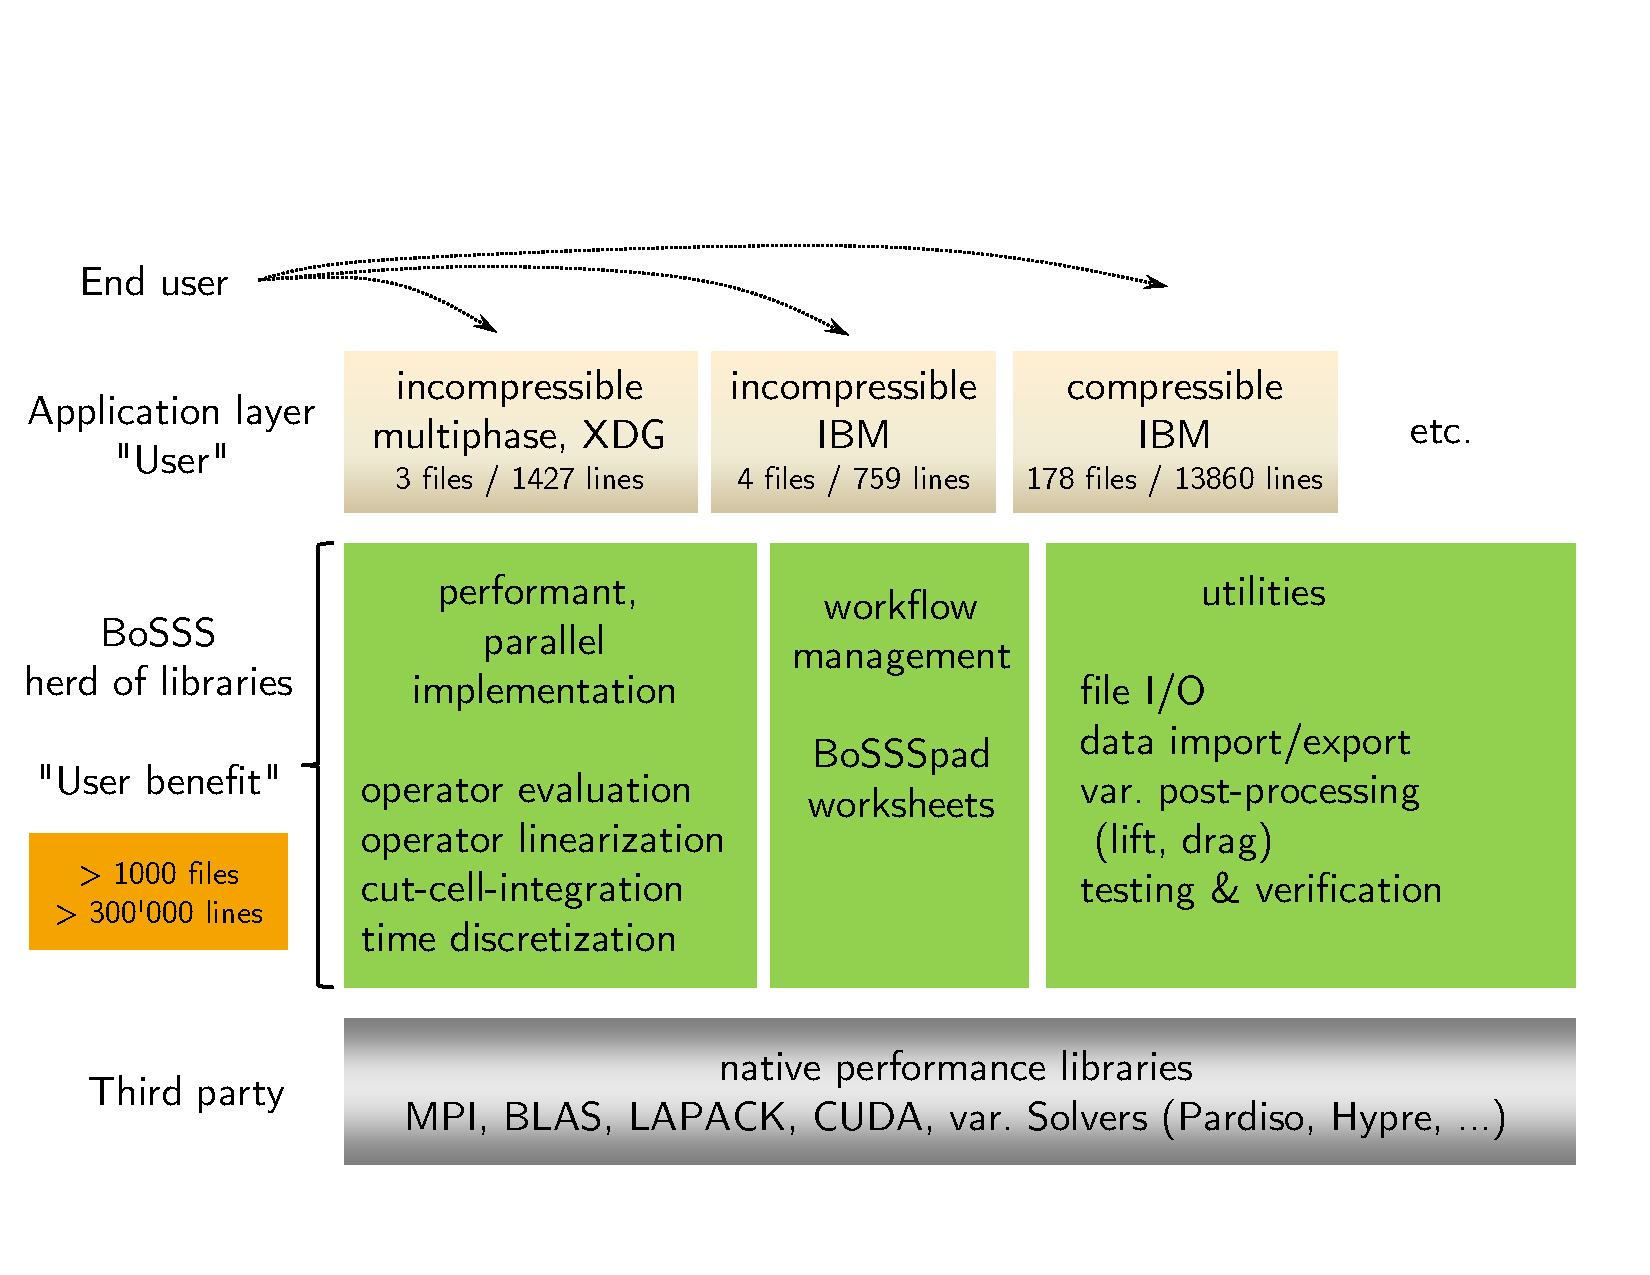
\includegraphics[width=\textwidth]{BoSSS-philosophy-1.pdf}
	\caption[Schematic representation of the structure of the BoSSS solver.]{Schematic representation of the structure of the BoSSS solver. Extracted from the BoSSS handbook \parencite{kummer2020}.}
	\label{Fig:BoSSS}
\end{figure}

